\documentclass[12pt,oneside]{uhthesis}
\usepackage{subfigure}
\usepackage[ruled,lined,linesnumbered,titlenumbered,algochapter,spanish,onelanguage]{algorithm2e}
\usepackage{amsmath}
\usepackage{amssymb}
\usepackage{amsbsy}
\usepackage{caption,booktabs}
\usepackage{ulem}
\captionsetup{ justification = centering }
%\usepackage{mathpazo}
\usepackage{float}
\setlength{\marginparwidth}{2cm}
\usepackage{todonotes}
\usepackage{listings}
\usepackage{xcolor}
\usepackage{multicol}
\usepackage{graphicx}
\usepackage{hyperref}
\usepackage{listings}
\floatstyle{plaintop}
%\restylefloat{table}
\addbibresource{Bibliography.bib}
% \setlength{\parskip}{\baselineskip}%
\renewcommand{\tablename}{Tabla}
\renewcommand{\listalgorithmcfname}{Índice de Algoritmos}
%\dontprintsemicolon
\SetAlgoNoEnd

\definecolor{codegreen}{rgb}{0,0.6,0}
\definecolor{codegray}{rgb}{0.5,0.5,0.5}
\definecolor{codepurple}{rgb}{0.58,0,0.82}
\definecolor{backcolour}{rgb}{0.95,0.95,0.92}

\lstdefinestyle{mystyle}{
    backgroundcolor=\color{backcolour},   
    commentstyle=\color{codegreen},
    keywordstyle=\color{purple},
    numberstyle=\tiny\color{codegray},
    stringstyle=\color{codepurple},
    basicstyle=\ttfamily\footnotesize,
    breakatwhitespace=false,         
    breaklines=true,                 
    captionpos=b,                    
    keepspaces=true,                 
    numbers=left,                    
    numbersep=5pt,                  
    showspaces=false,                
    showstringspaces=false,
    showtabs=false,                  
    tabsize=4
}

\lstset{style=mystyle}

\title{Sistema de Autenticación Central}
\author{\\\vspace{0.25cm}Nadia Gonz\'alez Fern\'andez}
\advisor{\\\vspace{0.25cm}Lic. Roberto Marti Cedeño}%\\\vspace{0.2cm}Lic. Juan José Roque Cires}
\degree{Licenciado en Ciencia de la Computación}
\faculty{Facultad de Matemática y Computación}
\date{Noviembre de 2022\\\vspace{0.25cm}\href{https://github.com/nala7/central_authentication_system}{github.com/nala7/central\_authentication\_system}}
\logo{Graphics/uhlogo}
\makenomenclature

\renewcommand{\vec}[1]{\boldsymbol{#1}}
\newcommand{\diff}[1]{\ensuremath{\mathrm{d}#1}}
\newcommand{\me}[1]{\mathrm{e}^{#1}}
\newcommand{\pf}{\mathfrak{p}}
\newcommand{\qf}{\mathfrak{q}}
%\newcommand{\kf}{\mathfrak{k}}
\newcommand{\kt}{\mathtt{k}}
\newcommand{\mf}{\mathfrak{m}}
\newcommand{\hf}{\mathfrak{h}}
\newcommand{\fac}{\mathrm{fac}}
\newcommand{\maxx}[1]{\max\left\{ #1 \right\} }
\newcommand{\minn}[1]{\min\left\{ #1 \right\} }
\newcommand{\lldpcf}{1.25}
\newcommand{\nnorm}[1]{\left\lvert #1 \right\rvert }
\renewcommand{\lstlistingname}{Ejemplo de código}
\renewcommand{\lstlistlistingname}{Ejemplos de código}


\begin{document}

\frontmatter
\maketitle


\begin{dedication}
    Dedicación
\end{dedication}
\begin{acknowledgements}
	A mi familia, que a pesar de la distancia siempre está muy cerca de mi. A mis padres, por siempre priorizar mi felicidad y mi bienestar. Gracias por sus sacrificios, ejemplo y amor, a ellos les debo la persona que soy hoy. A mi hermana, Laila, mi guía y mejor compañía. Mi primera profesora, la que me enseñó a sumar y restar y la que me enamoró de esta carrera. Gracias por tu paciencia y por siempre estar allí. A Mario, por hacerme sentir parte de su familia. A mis abuelos, por sus mimos. A mis tíos, Raisa, Olguita y Víctor por todas las aventuras. A mis primos, Iván, Mayte, Thalía y Vitico, por las horas de juego y alegría.
	
	A Luis, por ser mi constante y mi impulso cuando hacía falta. Por estar en las buenas y en las malas. Por elegir pasar esta experiencia a mi lado.
	
	A mis compañeros de cinco años de carrera. A Judy, Jose, Labourdette, Carlos, Sandra, Amalia, Gaby y Ariel por las largas madrugadas de proyectos y estudio, por las fiestas y las risas. A mis amigos, por hacer esta experiencia inolvidable.
	
	A mis profesores, por su dedicación y enseñanzas. A ellos les debo la profesional que hoy puedo decir que soy. A mi tutor, Roberto, por asumir esta tesis y todo el tiempo dedicado.
\end{acknowledgements}
\begin{opinion}
    Opiniones de los tutores
\end{opinion}
\begin{resumen}
	Resumen en español

%	Authentication is crucial although if system which facilitates secure their networks by limiting access to protected resources such as networks, websites, network-based software, databases, and other computer systems or services to only authenticated users (or processes). In general, modern authentication protocols such as Security Assertion Markup Language 2.0 (SAML), WS-Fed, OAuth, and OpenID discourage apps from handling user credentials. The aim is to keep an app's authentication method and its functionality separate. Azure Active Directory (Azure AD) manages the login process to keep confidential data (such as passwords) out of the hands of websites and apps. This allows identity providers (IdP) like Azure AD to provide seamless single sign-on experiences, allow users to authenticate using factors other than passwords (phone, face, biometrics), and block or elevate authentication attempts if Azure AD detects, for example, that the user's account has been compromised or that the user is attempting to access an app from an untrusted location. The main goal of the work is Converting Visual Studio from ADAL to MSAL has allowed us to better support Conditional Access and Multi-factor Authentication and other new AAD features which benefit our customers. Visual Studio 2019 and the.NET Core SDK can be used to complete this work. The SAML request–response authentication workflow between these providers is checked to ensure that user login information is accurate and safe.

\end{resumen}

\begin{abstract}
	Resumen en inglés
\end{abstract}
\tableofcontents
\listoffigures
% \listoftables
% \listofalgorithms
\lstlistoflistings

\mainmatter

\chapter*{Introducción}\label{chapter:introduction}
\addcontentsline{toc}{chapter}{Introducción}

%El Nodo Central es el responsable de todas las comunicaciones de la Universidad de La Habana. Presta servicios a todas las facultades, desde las que se encuentran en la Colina, hasta facultades externas como Economía, el Jardín Botánico y la Quinta de los Molinos. Servicios como Correo, acceso a Internet y proxy son  imprescindibles para garantizar el correcto funcionamiento de la institución. También es el encargado de proveer acceso a los estudiantes y trabajadores a todos los servicios digitales. Entre ellos se encuentra EVEA, el registro de notas, el sistema de contabilidad y el de recursos humanos. 

%Garantizar la seguridad de la información es uno de los mayores retos al que se enfrenta la institución actualmente.
%
%Una de las medidas de seguridad que se  utiliza es verificar  la identidad de los usuarios a través de un usuario y una contraseña  para acceder a los sistemas locales. Es importante que la autenticación del usuario sea correcta para que la aplicación permita un acceso correspondiente al rol de cada usuario.
%
%Todos los sistemas se han realizado de forma independiente a lo largo el proceso del digitalización de la Universidad. Todos tienen formas de acceso diferentes, lo cual significa que los usuarios para consumir los distintos servicios que utiliza diariamente tiene que autenticarse en cada de forma independiente. Esto crea dificultades tanto para los usuarios como para el Nodo Central. 

%Mecanismos de autenticación como el clásico usuario/contraseña son poco seguros o inadecuados, y más aún cuando los usuarios deben de acceder a cada aplicación por separado, ya que estas tienen su propio sistema de autenticación. Esto hace más engorroso el proceso de gestión de identidades y permisos a medida que aumenta la cantidad de usuarios en la red y debilitando la seguridad de acceso a las aplicaciones comprometiendo la confidencialidad de los datos.
%
%La necesidad de que el cliente repita el ingreso de la contraseña cada vez que accede a un servicio trae consigo varias dificultades: tiempo prolongado al tener que registrarse en varios sistemas para consultar información, la ubicación del servidor en una máquina remota implica inseguridad. Cuando la red crece mucho porque se encuentran una gran cantidad de usuarios conectados, puede volverse muy complejo el proceso de autenticación, es decir que es afectada la escalabilidad.
%
%Debido a esto se hace necesaria la gestión de la autenticación mediante la utilización de mecanismos que agilicen este proceso, sin que cause perdida de información, seguridad, confidencialidad o disponibilidad y que faciliten la gestión de grandes volúmenes de usuarios reduciendo el riesgo de caída de las aplicaciones y garantizando la gestión de identidades con el aumento de la seguridad, preferentemente con el uso de sistemas de identidad unificados


Hoy en día las personas utilizan muchos aplicaciones con distintas identidades. La identidad del usuario es considerada un conjunto de atributos, permanente o de larga vida, asociados a un usuario. Para obtener acceso a servicios muchas aplicaciones requieren que el usuario esté registrado y haya iniciado sesión. La mayoría de las veces los usuarios están registrados en distintos sitios o servicios con el mismo nombre de usuario y con la misma o similar contraseña, lo cual no es la mejor práctica para preservar la seguridad de las cuentas. Por todo ello el manejo de múltiples nombres de usuarios y contraseñas es una tarea molesta del Internet actual.

Teniendo en cuenta todos esos problemas de seguridad, cada vez más los administradores de sitios web deciden delegar esos servicios de administración y autenticación a terceros, entidades externas especializadas en ese tipo de actividad, que pueden alojar, almacenar, administrar y proteger los datos de los usuarios de un proveedor de servicios en particular. Además, ofrecen una interfaz de programación de aplicaciones (conocida también por la sigla API, en inglés, \textit{Application Programming Interface}), para proporcionar acceso a los datos del usuario a las aplicaciones externas. Estas soluciones permiten compartir los datos con más de un sistema web, permitiendo así el Inicio de Sesión Único (SSO) para aplicaciones de terceros.[\cite{kutera2016single}]

El Nodo Central de la Universidad de La Habana tiene entre sus responsabilidades dar las credenciales digitales a todos los usuarios de la Universidad. Los trabajadores y estudiantes de la institución registran sus datos personales en las bases de datos de recursos humanos y secretaria docente, respectivamente. Esa información es utilizada más adelante para que los usuarios puedan autenticarse en los distintos servicios de la institución, respaldado por sus sistemas de origen.

En este trabajo se presenta una solución a los problemas de autenticación que se ajusta a las necesidades y posibilidades de la Universidad de La Habana.  

\section*{Motivación}
Actualmente vivimos en un mundo donde la tecnología tiene un papel protagónico. La Universidad de La Habana en los últimos años ha estado inmersa en el proceso de transformación digital que lleva a cabo nuestro país, como continuidad de la estrategia de informatización de la sociedad cubana, que pretende integrar las tecnologías digitales a todos los ámbitos de la sociedad.

%En este sentido, nuestra sede universitaria ha avanzado en la digitalización de la información y los procesos y trabaja para facilitar el acceso a la red de todos sus estudiantes y trabajadores. A la par de estos avances, debe crecer también la seguridad de los sistemas para evitar brechas de información y asegurar la privacidad de los usuarios.

Garantizar un acceso seguro y sencillo a los recursos de la red es esencial para alcanzar este objetivo. Por consiguiente, se deben establecer mecanismos que cuenten con un alto nivel de seguridad y permitan identificar quién realmente está autorizado para acceder a los recursos del sistema.


%Nota Carmen: en que radica la mejora de la experiencia?????  para mi esto sobra a menos que digas en que mejora
%La creación de una plataforma central de autenticación resolvería muchos de estos problemas y mejoraría la experiencia de los usuarios. Estos solo tendrían una cuenta para acceder a todos los servicios que ofrece la Universidad, por lo que no tendrían que lidiar con formularios de inicio de sesión cada vez que vayan a acceder a un servicio.


\section*{Antecedentes}
%\textcolor{red} {Nota: Qué existe desde el punto de vista actual para autentificarte como usuario UH y sobre que esta soportado? qué problema trae ese soporte? existe en el mundo otros que pueden mejorar esas dificultades? Poner ejemplos. }

Actualmente todos los usuarios de la Universidad de La Habana se almacenan en dos Protocolos Ligeros de Acceso a Directorios (en inglés: \textit{Lightweight Directory Access Protocol}, también conocido por sus siglas como LDAP). En los dos directorios se guardan las cuentas de correo y los datos de sus usuarios. En uno ellos se registra la información de los estudiantes y en el otro la de los trabajadores. A partir de estos, todos los sitios web y aplicaciones de la universidad, individualmente, verifican la pertenencia del usuario a la institución.

Cada aplicación y servicio tiene un servicio de autenticación individual que dependen de los dos mencionados directorios que contienen a los usuarios.

\section*{Problemática}
La Universidad brinda servicios como Wi-Fi, correo, proxy y EVEA (Entorno Virtual de Enseñanza Aprendizaje), imprescindibles para el funcionamiento de la institución. También brinda servicios más especializados como los sistemas de contabilidad, recursos humanos, inventarios, el registro de notas, entre otros. Todos estos servicios utilizan la autenticación de forma individual, lo cual significa que un usuario tiene diversas cuentas a pesar de pertenecer todas a la misma institución.

El sistema implementado actualmente es poco eficiente y requiere de intervención humana constante para corregir y/o restablecer el apropiado funcionamiento de los servicios de autenticación. Esto genera tiempos elevados de respuesta y dificulta el mencionado proceso de transformación digital que está siendo llevado a cabo por nuestra Universidad.

\textcolor{red}{\section*{Hipotesis}}

\section*{Objetivo}
Con el propósito de presentar una propuesta para solucionar la problemática expuesta anteriormente, se plantean los siguientes objetivos:

\subsubsection*{Objetivo General}

\begin{itemize}	
	\item Diseñar e implementar un sistema de autenticación centralizada para todos los usuarios de La Universidad de La Habana. 
\end{itemize}

\subsubsection*{Objetivos Específicos}
\begin{itemize}	
	\item Generar los servicios de autenticación con compatibilidad con todas las tecnologías existentes y previstas en la institución.
	\item Implementar la gestión de control de acceso a todos los servicios ofrecidos por el Nodo Central de forma extensible a futuros servicios y fuentes de datos.
\end{itemize}

\section*{\textcolor{red}{Estructura de la Tesis}}
%\textcolor{blue}{Aca realmente toca hablar de como has organizado la tesis. De cada capítulo que tema toca, sus secciones y siempre un poco de información al respecto}




\chapter{Estado del Arte}\label{chapter:state-of-the-art}
En este capítulo se brindan las definiciones de herramientas utilizadas para la autenticación. También se realiza un estudio sobre el estado del arte de las mismas. Además, se brindan razones para incluir su utilización como parte de la solución propuesta.

\section{Inicio de Sesión Único}
El Inicio de Sesión Único ( en inglés \textit{Single Sign-On} o también conocido por sus siglas SSO) ha sido ampliamente adoptado para la autenticación en línea debido a su utilidad y seguridad que ofrece. Este es un método de autenticación que permite a los usuarios iniciar sesión con un único conjunto de credenciales en varios sistemas de software independientes. El inicio de sesión único facilita que un usuario no tenga que iniciar sesión en cada aplicación que use. Con este servicio los usuarios pueden acceder a todas las aplicaciones necesarias sin tener que autenticarse con otras credenciales.[\cite{microsoft-doc}]

En el mundo digital actual, los usuarios acceden a múltiples sistemas para llevar a cabo sus quehaceres. A medida que aumenta la cantidad de sistemas, también aumenta la cantidad de credenciales de cada usuario y, por lo tanto, también incrementa la posibilidad de perderlas u olvidarlas. El inicio de sesión único se puede utilizar para resolver muchos problemas relacionados con múltiples credenciales para diferentes aplicaciones. El acceso de inicio de sesión único al centro de autenticación principal permite a los usuarios obtener acceso a todos los demás recursos disponibles. SSO ayuda a mejorar la productividad del usuario y del desarrollador al evitar que el usuario recuerde varias contraseñas y también reduce la cantidad de tiempo que el usuario dedica a escribir varias contraseñas para iniciar sesión. SSO también simplifica la administración mediante la gestión de credenciales únicas en lugar de múltiples credenciales. Facilita la gestión de los derechos de un usuario que llega, cambia de función dentro o sale de la empresa, para integrar rápidamente aplicaciones adicionales, delegar derechos de acceso durante las vacaciones sin aumentar la carga de trabajo de la mesa de ayuda. [\cite{radha2012survey}]

Grandes empresas como Google, Facebook y Microsoft utilizan estos servicios. En particular Google permite a sus usuarios iniciar sesión una única vez para tener acceso a todos los servicios de la empresa que se encuentran en la nube. Cuando se configura SSO, los usuarios pueden iniciar sesión en terceros proveedores de identidad y luego acceder a las aplicaciones de Google directamente sin un segundo inicio de sesión [\cite{google-support}]. Por ejemplo, si se accede a un servicio de Google como Gmail, se autentica automáticamente en YouTube, AdSense, Google Analytics, y otras applicaciones de Google. Del mismo modo, si cierra la sesión de su Gmail u otras aplicaciones de Google, se cerrará automáticamente la sesión de todas las aplicaciones; esto se conoce como Cierre de Sesión Único (en inglés: \textit{Single Logout}) [\cite{sso-doc}]

%\subsection{Tipos de Inicio de Sesión Único}
%The various types of SSO shown in Fig: 1, fall under different categories, based on where they are deployed (Intranet, Extranet, Internet); how they are deployed (architecture – Simple, Complex); the credentials they use (token, certificate..) and the protocols they use (Kerberos, SAML, OpenID..).Following picture shows the types of SSO and their classification: 
%
%\begin{figure}[H]
%	\centering
%	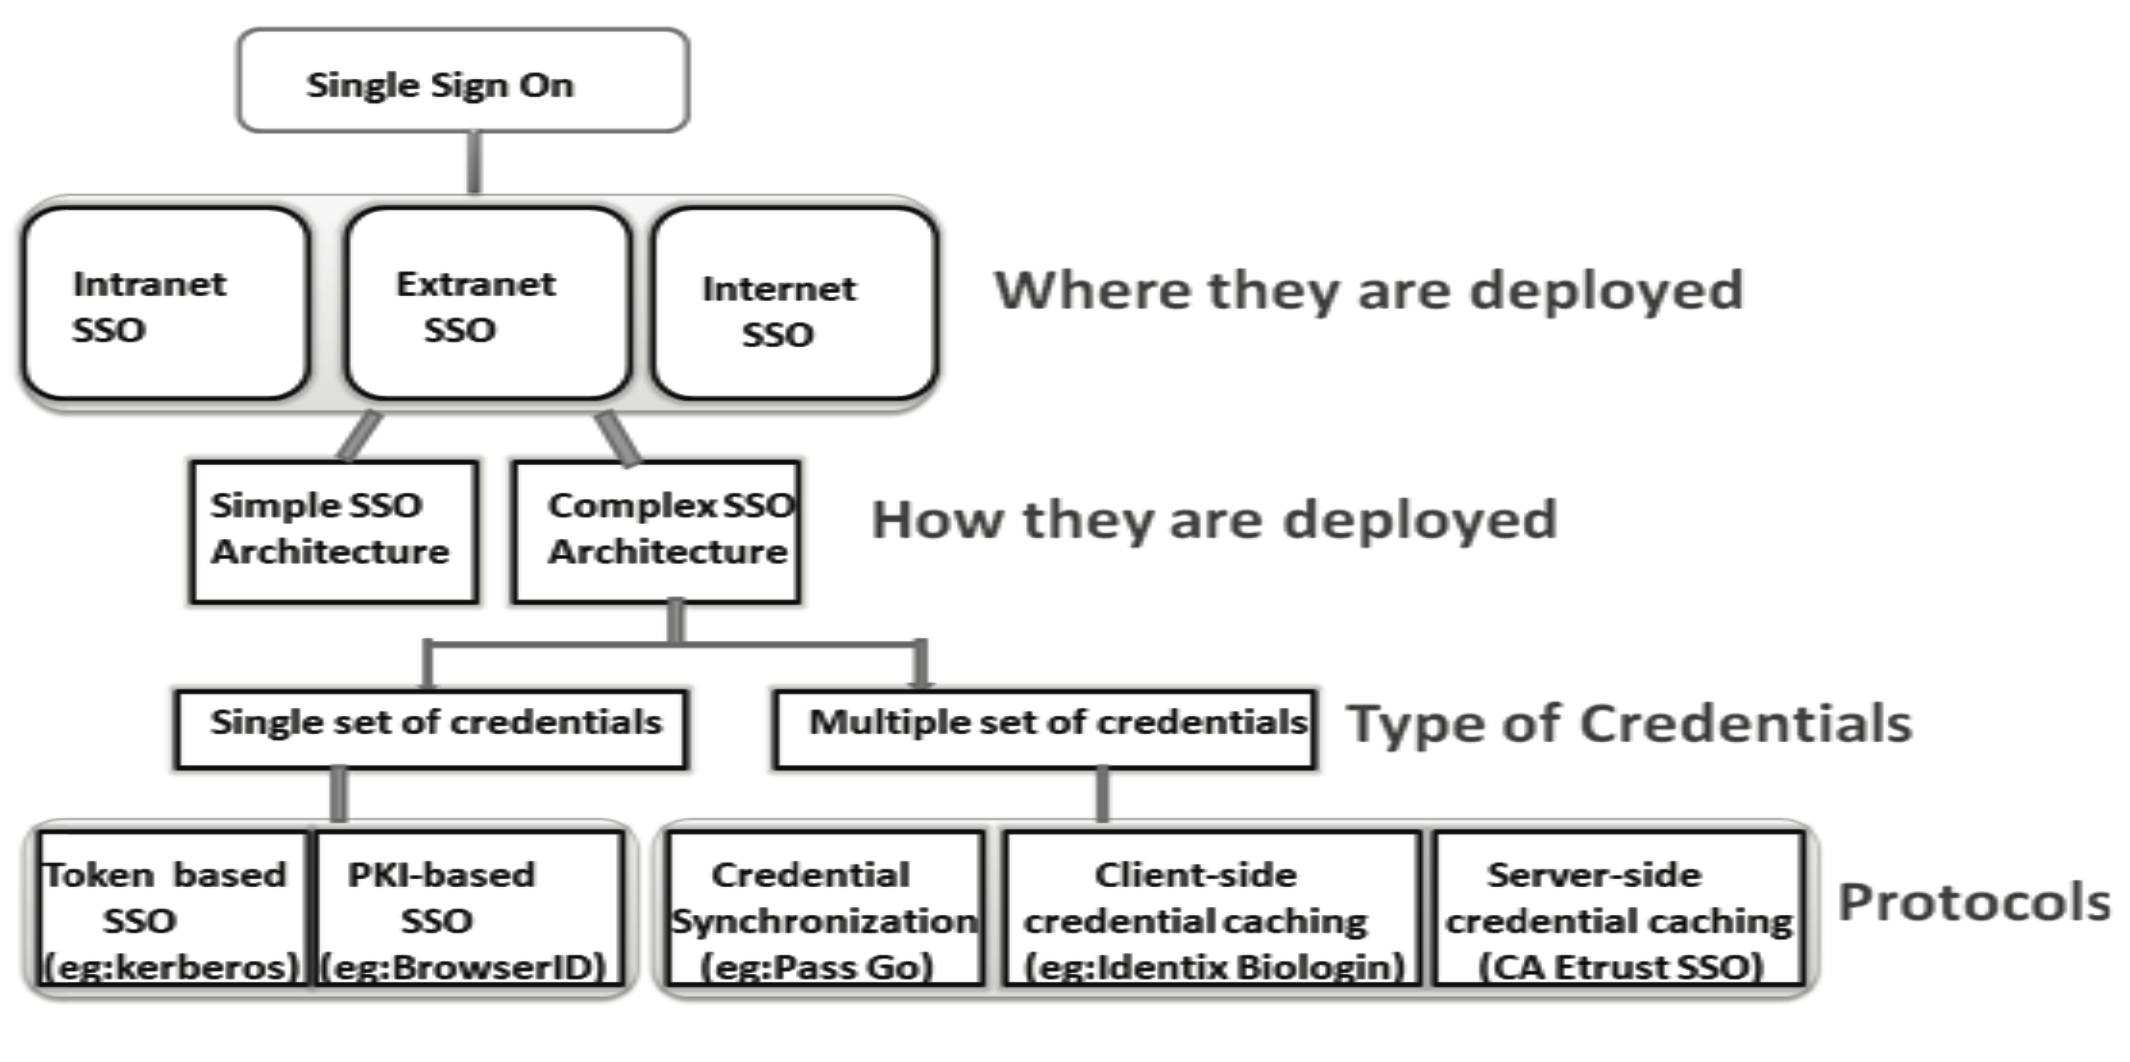
\includegraphics[width=0.7\linewidth]{Graphics/sso_types}
%	\caption{}
%	\label{fig:Tipos de SSO}
%\end{figure}
%
%Dadas las condiciones de la Universidad, se despliegará en Extranet ya que \textcolor{red}{Multi-domain SSO allows connecting to multiple systems within the same enterprise and all the business partners’ applications. The user can login into one enterprise and access resources of the other, the users need not login again using different credentials.}
%
%Se despliegará con una arquitectura de tipo SSO compleja ya que \textcolor{red}{Complex SSO uses multiple authentication authorities with single or multiple sets of credentials for each user.}
%
%En este caso se utilizarán un único conjunto de credenciales basado en tokens porque \textcolor{red}{In this SSO system, a user submits the credentials to the token-based authentication authority, in which the credentials have been checked with its credential database. If the user credentials match, then the user is returned with a token. When the user wants to access an application server which is governed by second authentication authority, the same token is delivered to get a ticket to access the application server. Success of this process relies on the trust the authentication authorities have among themselves.}

[\cite{radha2012survey}]

\section{OpenID Connect}
\textit{OpenID Connect}  (también OIDC)es una capa de identidad simple implementada a partir del protocolo \textit{OAuth 2.0}. Permite a los clientes verificar la identidad del usuario final en función de la autenticación realizada por un servidor de autorización, así como obtener información básica del perfil del Usuario final de manera interoperable y similar al protocolo REST. [\cite{openid-doc}]. 

\textit{OpenID Connect }es uno de los protocolos de tipo \textit{Single Sign-On} más utilizados para delegar la autenticación. También tiene un formato simple, por lo que ha ganado popularidad y es soportado por grandes empresas como Google, IBM, Microsoft, Amazon y PayPal [\cite{mainka2017sok}]. La nueva versión es compatible con \textit{API} y puede ser usado por aplicaciones nativas y móviles. También define mecanismos opcionales más robustos para firmas y cifrados. [\cite{openid-doc}]

Este protocolo está basado en \textit{OAuth 2.0} por lo que tiene todas las ventajas de este protocolo. Sin embargo, lo extiende ya que ofrece facilidades para obtener más información de la identidad de los usuarios eficientemente. Permite un flujo de información adicional que genera un \textit{id-token} que contiene datos del usuario. De esta forma las aplicaciones no solo tienen acceso a los permisos de los usuarios, sino también obtienen información sobre la identidad de los usuarios.  [\cite{openid-doc}][\cite{kutera2016single}]

\section{Otros protocolos de autenticación}
\subsection{SAML}
Lenguaje de Marcado para Confirmaciones de Seguridad, conocido como SAML (en inglés: \textit{The Security Assertion Markup Language}) es un marco de trabajo que permite expresar asertos\footnote{ Los asertos definen las afirmaciones de seguridad de una entidad dentro de un sistema. Estas afirmaciones pueden ser de tres tipos: asertos de autenticación, de atributos y de decisiones de autorización.} acerca de la identidad, los atributos y las autorizaciones de un sujeto con el objetivo de facilitar las relaciones entre distintas empresas, así como las relaciones de estas con sus usuarios. Este marco de trabajo permite a las compañías crear identidades federadas, lo cual les facilita las tareas de gestión de perfiles, autenticación y autorización de usuarios. El caso típico de uso es el de \textit{Single-Sign-On }(SSO), que permite a los usuarios acceder a diversos sitios en la federación con una única autenticación. [\cite{sanchez2009estudio}]

SAML y OpenID Connect son protocolos de identificación, diseñados para autenticar a los usuarios. También proporcionan datos de identidad para el control de acceso y como método de comunicación para la identidad de un usuario.

SAML durante muchos años ha proporcionado un medio seguro de intercambio de datos de identidad, por lo que muchas organizaciones confían en él. También es muy rico en funciones y cubre una amplia gama de requisitos de identidad.


OIDC, al ser más nuevo y en se encuentra desarrollo, todavía está rezagado con respecto a SAML en términos de características. Sin embargo, para muchas aplicaciones donde solo se necesita un requisito simple para los datos de identidad básicos, particularmente en el espacio del consumidor, OIDC es muy útil, ya que es mucho más fácil de usar que SAML y no requiere el manejo pesado de XML que requiere SAML.

Actualmente, SAML se usa prinipalmente para la identificacion de ciudadanos del gobierno y la autenticación empresarial. Sin embargo, esto está comenzando a cambiar, con sistemas más modernos que utilizan OIDC en lugar de SAML. Esto se debe a que OIDC permite un procesamiento de datos más liviano que SAML, utilizando tokens JSON (token de ID) en lugar de XML. OIDC es ideal para usar con aplicaciones móviles y aplicaciones web de una sola página, donde el uso de SAML sería complicado. [\cite{naik2017securing}]

OIDC se adapta a las condiciones del Nodo Central de la Universidad de La Habana ya que se cuentan con pocos recursos, por lo que es necesario un procesamiento ligero de información. 

\subsection{Kerberos}
Kerberos es una conexión de software que se emplea en una red grande para establecer la identidad declarada de un usuario. Utiliza una combinación de encriptación y Bases de Datos distribuidas de tal forma que un usuario pueda registrarse y comenzar una sesión desde cualquier computadora localizada en la red mediante la obtención de tickets para servicios de un servidor especial conocido como TGS (servidor despachador de tickets); cada ticket contiene información para identificar al usuario o servicio encriptada con la clave privada para el servicio. Como sólo Kerberos y el servicio conocen dicha clave, se considera que el mensaje está genuinamente originado en la fuente y que no fue adulterado en el transporte del mismo. El ticket otorgado por el TGS contiene una nueva clave de sesión que solo conoce el cliente y el servicio afectado. Esta clave será utilizada para encriptar las transacciones que ocurren durante la sesión.
Una de las ventajas es que el ticket tiene un tiempo de vida específico, y una vez que éste expira, debe solicitarse un nuevo ticket al TGS para poder seguir utilizando el servicio. Para cada servicio se requiere un ticket distinto. Otra ventaja es que el usuario no debe reingresar la password cada vez que requiere un servicio, porque si el ticket TGS no expiró puede reusarlo para pedir otro ticket de servicio deseado. Por este motivo, el tiempo de vida del ticket TGS deberá ser mayor que el tiempo de vida del ticket de servicio.


\section{LDAP}
El Protocolo Ligero de Acceso a Directorios (en inglés: \textit{Lightweight Directory Access Protocol}, también conocido por sus siglas de LDAP) es un conjunto de protocolos de licencia abierta que son utilizados para acceder a la información que está almacenada de forma centralizada en una red. Este protocolo se utiliza a nivel de aplicación para acceder a los servicios de directorio remoto. [\cite{ldap-doc}]

LDAP está basado en estándares implementados sobre TCP/IP. Permite a los clientes interactuar directamente con los servidores de los directorios: almacenar y consultar información, buscar datos filtrados, autenticar usuarios, entre otros.

Este protocolo es utilizado actualmente por muchos sistemas que apuestan por el software libre al utilizar distribuciones de Linux para ejercer las funciones propias de un directorio activo en el que se gestionarán las credenciales y permisos de los usuarios y estaciones de trabajo en redes LAN corporativas en conexiones cliente/servidor.

Un directorio remoto es un conjunto de objetos que están organizados de forma jerárquica, tales como: nombre, claves, direcciones, etc. Estos objetos estarán disponibles para una serie de clientes conectados mediante una red, normalmente interna o LAN, y proporcionarán las identidades y permisos para esos usuarios que la utilicen.

LDAP está basado en el protocolo X.500 para compartir directorios, y contiene esta información de forma jerarquizada y mediante categorías para proporcionarnos una estructura intuitiva desde el punto de vista de la gestión por parte de los administradores.

Estos directorios se utilizan generalmente para contener información virtual de usuarios, para que otros usuarios accedan y dispongan de información acerca de los contactos que están aquí almacenados. Además es capaz de comunicarse de forma remota con otros directorios LDAP situados en servidores que pueden estar en el otro lado del mundo para acceder a la información disponible. De esta forma se crea una base de datos de información descentralizada y completamente accesible.
 
El sistema de autenticación vigente en el Nodo Central verifica sus usuarios con dos sistemas implementados con LDAP. Este protocolo se adapta a las necesidades y condiciones actuales de la Universidad ya que es \textit{Open Source} (OSS o código abierto).
%\textcolor{red}{
%	- It is a mature, flexible, and well supported standards-based mechanism for interacting with directory servers. It’s often used for authentication and storing information about users, groups, and applications, but an LDAP directory server is a fairly general-purpose data store and can be used in a wide variety of applications. \\ LDAP is a tool in the User Management and Authentication category of a tech stack.}


\section{Active Directory}
Directorio Activo (en inglés: Active Directory, conocido también por sus siglas AD) es un servicio de directorios desarrolado por Microsoft que permite almacenar información como usuarios y dispositivos en una base de datos centralizada y jerárquica. AD brinda servicios como autenticación, políticas de acceso y administración de grupos.

Active Directory almacena información sobre objetos en la red y hace que esta información sea fácil de encontrar y usar para administradores y usuarios. Active Directory utiliza un almacén de datos estructurados como base para una organización lógica y jerárquica de la información del directorio.

La seguridad está integrada con Active Directory a través de la autenticación de inicio de sesión y el control de acceso a los objetos del directorio. Con un solo inicio de sesión en la red, los administradores pueden administrar los datos del directorio y la organización en toda su red, y los usuarios autorizados de la red pueden acceder a los recursos en cualquier lugar de la red. La administración basada en políticas facilita la gestión incluso de la red más compleja.
[\cite{active-directoy-doc}]

\begin{table}[H]
	\centering
	\begin{tabular}{ |p{4cm}||p{4cm}|p{4cm}| }
		\hline
		 &\textbf{LDAP}&\textbf{AD}\\
		\hline
		\textbf{Nombre Completo }  &  Protocolo Ligero de Acceso a Directorios  &Directorio Activo\\
		\hline
		\textbf{Función}& Protocolo&Proveedor de servicios de directorios\\
		\hline
		\textbf{Standard} &Código Abierto & Propietario\\
		\hline
		\textbf{Sistemas Soportados}&Multiplataforma: Windows, Linux, macOS & Para aplicaciones y usuarios de Windows\\
		\hline
		\textbf{Uso principal}&   Consultar y modificar elementos en proveedores de servicios de directorio & Proveer autenticación, políticas, administración de grupos y usuarios, y muchos otros servicios en forma de una base de datos de directorio\\
		\hline
	\end{tabular}
	\caption{\label{tab:table-name}Comparación entre LDAP y Active Directory.}
\end{table}

\section{Okta}

\section{Gluu}
Gluu es una plataforma de código abierto gratuita que proporciona a las organizaciones un servicio de autenticación y autorización para las aplicaciones web y móvil. Permite configurar SSO (Single Sign-On) en aplicaciones que tengan soporte para OpenID Connect, SAML o  CAS para identidades federadas.

\section{Auth0}
Auth0 es una plataforma en la nube que ofrece la autenticación y la autorización como un servicio. Auth0 dispone de herramientas para simplificar la autenticación de las aplicaciones y APIs ya que hace uso de estándares como OAuth2.0, OpenID Connect, SAML 2.0, JSON Web Token o WS-Federation, ofreciendo SSO (Single Sign-On) a entornos empresariales

\section{Keycloak}
Keycloak es un software de código abierto que permite el \textit{Single Sign-On} o Inicio de Sesión Único con \textit{Identity Management} y \textit{Access Management} para aplicaciones y servicios modernos. Esta herramienta facilita la protección de aplicaciones y servicios con poca o ninguna codificación. Un Proveedor de identidad (en inglés: \textit{Identity Provider}, también conocido por sus siglas IdP), permite que una aplicación (a menudo llamada \textit{Service Provider} o SP) delegue su autenticación. [\cite{KeycloakDoc}]

Este software está escrito en Java y es compatible de forma predeterminada con los protocolos de federación de identidad SAML v2 y OpenID Connect (OIDC) / OAuth2. Está bajo licencia de Apache y es  mantenido por Red Hat. [\cite{KeycloakDoc}]

	\subsection{Características}
	Los usuarios se autentican en Keycloak en lugar de hacerlo en las aplicaciones. Esto significa que no es necesario que cada aplicación tenga un formulario de inicio de sesión, autentique a los usuarios o almacene sus datos. Una vez entren en Keycloak, los usuarios no tendrán que iniciar sesión en las demás aplicaciones conectadas al software.
	
	Lo mismo sucede cuando un usuario cierra sesión. Keycloak ofrece cierre de sesión único, lo cual significa que los usuarios solo tienen que desconectarse en una de las aplicaciones para salir de su cuenta en el resto. 
	
	Otra prestación de Keycloak son las federaciones de usuarios, que facilitan la compatibilidad con LDAP y otros servidores de directorios activos. También admite la implementación de servicios propios para usuarios guardados en otros tipos de almacenamientos como en bases de datos relacionales. 
	
	Keycloak ofrece como herramienta una consola de administración de cuentas, a través de la cual los usuarios pueden administrar sus propias cuentas. Pueden actualizar su perfil, cambiar sus contraseñas y configurar la autenticación en dos pasos. También pueden administrar sus sesiones y visualizar el historial de su cuenta. 
	
	Otra característica es que es una herramienta extensible porque permite la eliminación, adición y modificación de las bases de datos de usuarios, los métodos de autenticación y los protocolos. Está basada en protocolos estándares y soportan OpenID Connect, OAuth 2.0 y SAML. [\cite{KeycloakDoc}]
	
	Keycloak facilita añadir la autenticación y un servicio seguro a aplicaciones. Permite que los desarrolladores se centren en la funcionalidad empresarial al no tener que preocuparse por los aspectos de seguridad de la autenticación. También posibilita la unificación de los métodos de autenticación de distintas aplicaciones sin modificarlas.
	
%	\textcolor{red}{\textbf{Comparación}}
%	\textcolor{red}{Gluu: \\ Free open source access management suite with support for SAML and OpenID Connect SSO, and OAuth2 based web and API access management. The Gluu Server can include multiple components. Each one fulfills a different requirement, and can be included or excluded in individual deployments based on an organization’s unique requirements.}
%	\textcolor{red}{Gluu vs Keycloak: \\
%		- The Keycloak system requires 512 Mb of RAM and 1 GB of disk space, whereas the Gluu system requires 8 GB of RAM and 40 GB of disk space. \\ - Gluu is less flexible to extend} [\cite{vassallo2017continuous}]
Gluu es otra de las tecnologías que tienen prestaciones y ventajas similares a Keycloak. Es un servicio \textit{Open Source} que soporta \textit{SAML}, \textit{OpenID Connect, SSO} y \textit{OAuth 2.0}. Sin embargo Gluu es un sistema que requiere de 8 GB de RAM y 40 GB de espacio en disco, mientras que Keycloak solo necesita de 512 Mb de RAM y 1 GB de disco. Por ello Keycloak se ajusta más a los recursos que se tienen en la Universidad de La Habana.

\subsection{JSON Web Token}
\textit{JSON Web Token }(abreviado JWT) es un estándar abierto basado en JSON propuesto por IETF (RFC 7519) para la creación de tokens de acceso que permiten la propagación de identidad y privilegios [\cite{bradley_sakimura_jones_2015}].

Esta tecnología define una forma compacta y autónoma para transmitir de forma segura información entre las partes como un objeto JSON. Esta información es verificada y confiable ya que se encuentra firmada digitalmente. Los JWT se pueden firmar usando un secreto (con el algoritmo HMAC) o un par de claves públicas / privadas usando RSA.

JSON Web Token es un método compacto y autónomo para transmitir información, se basa en una cadena de texto que tiene 3 partes (Header, payload, signature) codificadas en Base64, separadas por un punto que es estregado a los clientes de una API como llave de acceso. Keycloak utiliza JWT para transmitir una llave secreta de acceso a usuarios con privilegios. [\cite{muyon2020metodos}]

\subsection{REST API}
Se utiliza API REST como medio de prueba para ejecutar peticiones HTTP que posteriormente serán aseguradas con un Json Web Token emitido por Keycloak. La arquitectura REST enfoca a todo lo que lo conforma como un recurso. Los servicios web REST son livianos, altamente escalables y mantenibles. Se usan muy comúnmente para el intercambio de información, es el estándar más lógico, eficiente y generalizado en la creación de API para servicios de internet.

El siguiente esquema muestra como se realiza el flujo de información para autenticarse a través de Keycloak:

\begin{figure}[H]
	\centering
	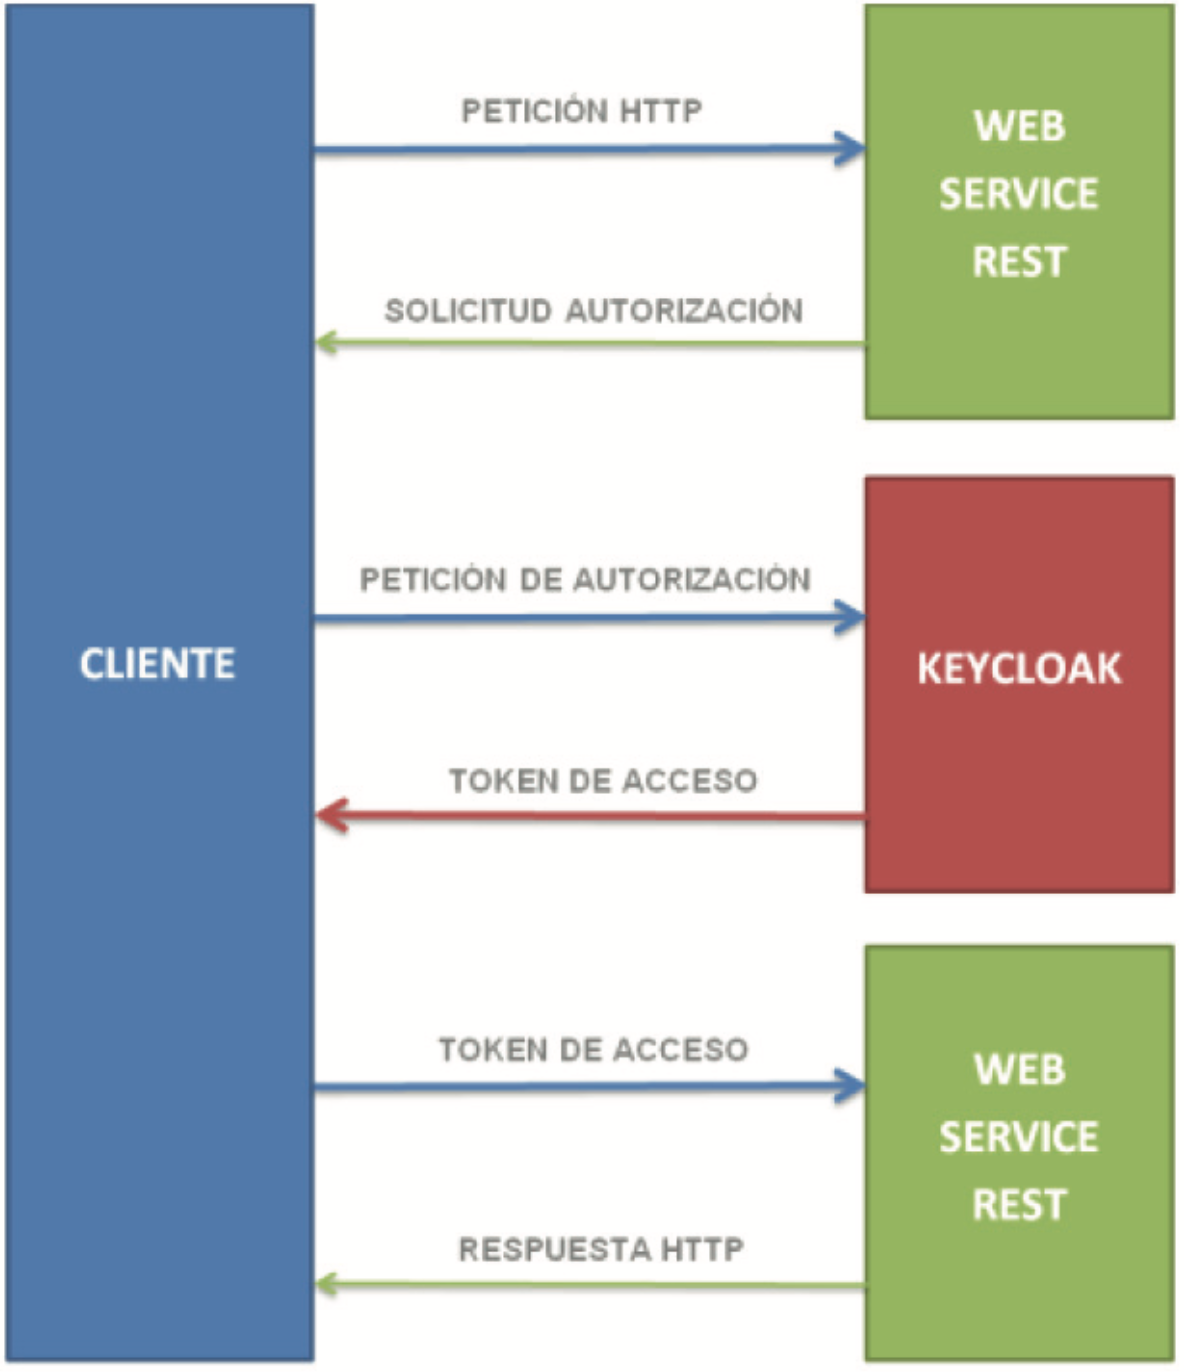
\includegraphics[width=0.7\linewidth]{Graphics/keycloak_info_flux}
	\caption{}
	\label{fig:Flujo de Información en Keycloak}
\end{figure}

Este flujo asegurar que solo los usuarios a los que se les otorgó el acceso al servicio web puedan consumir dicha API. De esta forma se evita el acceso no autorizado a información que se transmite bajo un protocolo no seguro como lo es el protocolo HTTP. [\cite{muyon2020metodos}]

\chapter{Propuesta de Sistema Central de Autenticación}\label{chapter:proposal}
En el siguiente capítulo (...)
\section*{Hipótesis}
La Universidad de la Habana cuenta con varios sistemas en la red donde se utiliza el método tradicional de usuario/contraseña como mecanismo de seguridad para acceder a diversas aplicaciones, este proceso de autenticación se hace muy complejo al tener que acceder a cada uno de ellos de forma independiente. Con cada servicio nuevo se debe crear un sistema de autenticación que garantice la seguridad de sus datos y se deben hospedar la información de los usuarios repetidas veces, lo cual utiliza una mayor cantidad de recursos y es más propenso fallas.

Para eliminar estas dificultades se realiza un sistema central de autenticación que se basa en el método Inicio de Sesión Único. Esta propuesta tiene como objetivo un aumento en la productividad, tener mayor facilidad de acceso a los recursos, funciones de autenticación a través de una única plataforma, una administración sencilla de credenciales y sobre todo garantizar un aumento de la seguridad. Mediante este servicio el usuario podrá registrarse en el sistema una sola vez, con lo cual podrá acceder a todos los recursos sin tener que volver a autenticarse.




\subsection*{Requisitos del Software:}
\begin{itemize}
	\item Unificar las distintas fuentes de datos.
	\item Que el usuario inicie sesión y, hasta que cierre sesión, sea capaz de realizar operaciones sin tener que volver a introducir credenciales. 
	\item El servicio ofrecido al cliente debe permitir que el usuario extienda la sesión una vez pasado el tiempo de expiración de la misma sin que volver a introducir credenciales. 
	\item Reconocer la identidad de los usuarios durante el proceso de autenticación para garantizar un adecuado control de acceso a recursos del sistema.
	\item Proteger los recursos del sistema, permitiendo que estos sean solamente usados por aquellos usuarios a los que se les ha concedido autorización.
	\item Que el usuario inicie sesión con dos únicos campos: nombre de usuario y contraseña. Este requisito será suficiente para garantizar la interoperabilidad del sistema, que debe ser capaz de generar un objeto encriptado con toda la información relativa a dicho usuario y viajar por la red de comunicaciones entre las distintas entidades. 
	\item  La respuesta obtenida al iniciar sesión de forma exitosa debe ser un objeto que le dé portabilidad y reusabilidad al software.
	\item En caso de obtener un inicio de sesión erróneo, retornar un error
	\item Garantizar el control de errores y excepciones.
	\item La evaluación de permisos de acceso
\end{itemize}

El software consta de varias etapas:

\begin{figure}[H]
	\centering
	\includegraphics[width=0.9\linewidth]{"Graphics/Diagrama Tesis"}
	\caption{}
	\label{fig:diagrama-tesis}
\end{figure}

\section*{Bases de Datos}

%que es
Actualmente los estudiantes de toda la Universidad de La Habana al matricularse se inscriben en secretaría en el Sistema de Gestión de la Nueva Universidad (SIGENU). En este sistema se almacenan todos los datos de los alumnos: datos personales, proveniencia, notas, grados.

Por otra parte, los datos de los profesores y resto de trabajadores de la Universidad son guardados en bases de datos de ASSETS, software contratado. Cada unidad presupuestada de la Universidad tiene su propio ASSET donde almacena los datos de recursos humanos y del inventario.

%problema
El Nodo Central es el responsable de todas las comunicaciones de la Universidad de La Habana. Presta servicios a todas las facultades, desde las que se encuentran en la Colina, hasta facultades externas como Economía, el Jardín Botánico y la Quinta de los Molinos. Cada facultad tiene su sistema independiente donde gestiona a todo su personal que responde a sus necesidades. 

La información es almacenada en varias bases de datos, lo cual hace difícil la gestión de todos los usuarios de la Universidad. Crear un sistema único al cual todas las facultades pudieran acceder de forma remota simplificaría el trabajo, no solo a los programadores , sino también a los usuarios. Por ejemplo, cada estudiante podría matricularse en su propia facultad y se evitarían las aglomeraciones y la confusión creada todos los años. 

Por otra parte sería complicado cambiar el software utilizado por toda. Como se  la institución. Como mencionó anteriormente, algunas facultades se encuentran alejadas de La Colina, lo cual dificulta la comunicación y la instalación de nuevos sistemas. También se debe tener en cuenta que la experiencia del usuario sería diferente con un nuevo software. El personal trabajador de la Universidad es de diversas edades, por lo que podría ser complejo la adaptación a una nueva interfaz.

% propuesta
Por lo tanto en el presente trabajo se ha decidido no cambiar los sistemas. La unificación de las bases de datos de usuario de toda la Universidad de La Habana es un proceso complejo que no se encuentra en los objetivos del presente trabajo. 

Por otra parte, se necesita un nombre de usuario único para cada trabajador y estudiante de la institución. Al utilizarse distintas fuentes de datos, no se puede garantizar que todas las bases de datos tengan las mismas estructuras. Sin embargo, todos los usuarios tienen una cuenta de correo que los identifica unívocamente, por lo que utilizar este campo como nombre de usuario garantiza que cada persona es identificado.

\section*{Ingestión de Datos}
La ingesta de datos es el proceso mediante el cual se introducen datos, de diferentes fuentes,
estructura o características dentro de otros sistemas de almacenamiento o procesamiento de
datos.  [\cite{fernandez2020aplicacion}]

Teniendo varias fuentes de datos, para garantizar una ingestión de datos exitosa, la solución debe ser capaz que leer información de distintas fuentes de datos. 

Por otra parte el estado de un usuario puede cambiar y sus permisos de acceso pueden variar. Por ejemplo, a los estudiantes se les puede dar de baja o un trabajador puede terminar su contrato y por lo tanto se les debe quitar sus credenciales de forma inmediata. Un estudiante después de graduarse puede pasar a se trabajador de la institución, por lo que sus permisos de acceso deben ser cambiados. Otro caso sería cuando un estudiante o trabajador sale una licencia, deben suspenderse sus credenciales temporalmente hasta que la persona regrese. 

Se necesita que el sistema de autenticación se actualice constantemente ya que las bases de datos cambian sus datos.

La Universidad  se encuentra en constante cambio. Por ejemplo, en 2017 culminó el proceso de adscripción del Instituto Superior de Diseño (ISDI) a la Universidad de La Habana [\cite{isdi-historia}]. Para ello fue necesario incorporar todos los datos de los usuarios del ISDI al sistema de autenticación vigente para otorgarles las credenciales correspondientes. Por ello, el nuevo sistema debe ser capaz de admitir nuevas fuentes de datos de forma sencilla en un futuro. 

En el nodo central, la ingesta de datos se hace a través de LDAP. \textcolor{red}{(explicar brevemente para qué se usa LDAP en el nodo y cómo ingesta los datos)}

\section*{Capa de Autenticación}
La autenticación es un área clave en la seguridad de la información. En la modernidad los usuarios necesitan acceder a muchos servicios digitales imprescindibles para su vida cotidiana. Las contraseñas basadas en caracteres alfanuméricos han sido las más comunes en todo tipo de sistemas por su fácil implementación. [\cite{rodriguez2018seguridad}]


El proceso de autenticación consiste en la verificación de la identidad de un usuario o una entidad  [\cite{teheran2014mecanismo}]. Los usuarios de la institución utilizan diariamente distintos servicios, que van desde acceder a Internet por la red WI-FI o por proxy, hasta servicios web como EVEA y correo. Cada servicio tiene su propio sistema de autenticación.

Resulta engorroso crearse una cuenta en cada uno de los sistemas y autenticarse cada vez que uno acceda a un sitio nuevo. La creación de un sistema en el cual todos los usuarios de la Universidad puedan autenticarse con su correo de la institución y su contraseña facilitaría la interacción diaria con los servicios ofrecidos por el Nodo Central.

Para ello se debe garantizar la seguridad de las cuentas. Por ejemplo, los estudiantes utilizan la máquinas de los laboratorios y se autentican con su cuenta personal. Es común que las personas olviden cerrar sus sesiones, por lo que la cuenta debe expirar al pasar de un tiempo prudencial, de lo contrario, su información puede ser utilizada por otra persona.



Se utilizará la autenticación basada en tokens ya que permite 

En este caso la capa de autenticación es la encargada de recibir las peticiones de los distintos clientes y verificar la identidad de un usuario a partir de la información recopilada por la Ingestión de datos.

\begin{figure}[H]
	\centering
	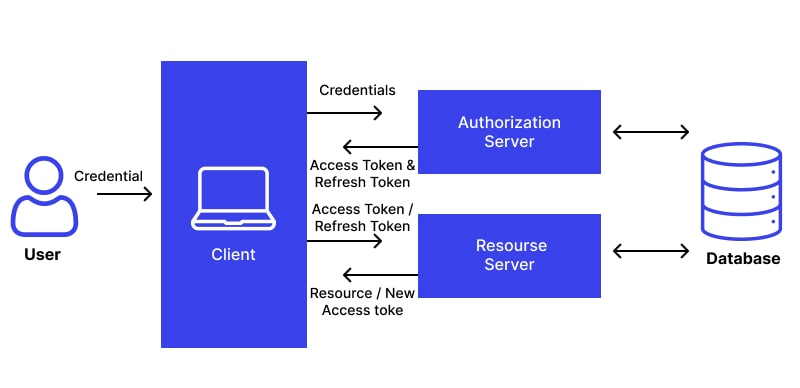
\includegraphics[width=0.9\linewidth]{Graphics/token-based-auth}
	\caption{}
	\label{fig:token-based-auth}
\end{figure}



\section*{Clientes}
El Nodo Central brinda infraestructura a los servicios de la Universidad vitales para el correcto funcionamiento de la institución. Entre responsabilidades se encuentran la gestión de correo, el acceso a Internet, las cuentas de usuarios y en el caso de los profesores gestión de cuentas de VPN. También tiene como clientes todos los servicios web de la casa de altos estudios, \textcolor{red}{entres ellos el sitio oficial de la Universidad https://www.uh.cu/, los sistemas utilizados en recursos humanos, en los departamentos de contabilidad}

Cada cliente tiene su propio sistema de autenticación, lo cual no es eficiente ya que utiliza una mayor cantidad de recursos porque cada uno tiene su registro de usuario en bases de datos individuales. También crea brechas de seguridad ya que no todos cumplen los estándares que deberían y existe más información en la red expuesta a ataques externos. 

El software debe ser capaz de admitir nuevos clientes fácilmente. 
Uno de los clientes más importantes es el Entorno Virtual de Enseñanza y Aprendizaje, más conocido como EVEA, creado en 2018. Este es una plataforma informática encargada de orientar la comunicación pedagógica entre los universitarios que intervienen en el proceso educativo. También, tiene la misión de crear espacios o comunidades organizadas en torno al estudio. [\cite{evea-cd}] 

Este entorno virtual representó un apoyo para el sistema universitario cuando los estudiantes no podían asistir a sus facultades debido a la pandemia provocada por la covid-19 en diciembre del 2019 [\cite{ferrer2020pandemia}] . En la primera mitad del año 2020 la cantidad de usuario aumentó considerablemente en poco tiempo. El sistema era lento y tenía muchas fallas. Uno de los mayores retos fue lograr registrar a todos sus usuarios y que estos se pudiera autenticar. De haber existido un sistema que ya autenticara a todos los estudiantes y profesores de la Universidad, los programadores habrían tenido un problema menos a la hora de modificar la plataforma para adaptarla al nuevo uso que se le daría.



\section*{Usuarios}


\textbf{Estructura del Cap 2}

\begin{itemize}
	\item Descartar otras opciones
	\item Describir brevemente por qué Keycloak (despues en mas detalle cada componente)
	\item Propuesta: Diagrama
	\\
	\item
	-	qué es la etapa/componente
	-	cuál es problema concreto
	-	propuesta de solución
	\\
	\item \textbf{	Bases de datos: }
	\\
	qué es: dónde y en qué formato se almacena la información\\
	problema: Hay muchas facultades, es dificil cambiar como se introducen los datos. \\
	propuesta: no cambiar nada, tiene que tener la base de datos una columna con valores únicos que pueda ser usado como nombre de usuario
	\\
	\item \textbf{Ingestión de datos}
	\\
	Qué es: definición
	problema:
	- Aceptar varias fuentes de datos\\
	- Actualizarse live. por si un estudiante se gradúa, un trabajador culmina su contrato, un trabajador empieza un contrato, un estudiante comienza primer año, estudiante pasa a ser trabajador, estudiante regresa de licencia.\\
	- Contraseña ?????\\
	- Añadir fuentes de datos dinámicamente\\
	propuesta: keycloak, why?
	\\
	\item \textbf{Capa de autenticación}\\
	Qué es: definición\\
	problema:\\
	- unificar\\
	- seguridad, computadoras compartidas en el laboratorio\\
	- refresh\\
	- logout, \\
	propuesta: keycloak (ya se está usando para ingestión de datos mantenimiento, simplicidad, facilidad de aprendizaje, menos recursos)
	\\
	\item \textbf{Clientes}\\
	Qué es: definición, en la UH: correo, evea\\
	Problema: todos distintos, nada en común, seguridad del sistema de autenticación\\
	Propuesta: que los servicios utilicen el API de keycloak para autenticar\\
	tu tesis no modifica los clientes existentes, pero ilustra cómo hacerlo con un cliente de ejemplo desarrollado en Python.\\
	\\
	\item \textbf{Usuarios}\\
	Qué es: personas jóvenes, personas mayores\\
	Problema: confuso\\
	\\
	\textcolor{red}{Los usuarios se ven obligados a tener más de unas credenciales lo cual crea confusión. Frecuentemente se olvidan los nombres de usuarios o contraseñas o se utilizan las mismas credenciales en varios sitios, lo cual es una mala práctica desde el punto de vista de la seguridad.}
	\\
	Propuesta: sus servicios no van a cambiar, pero única contraseña, seguridad añadida sin cambiar la experiencia de usuario
	
\end{itemize} 


\chapter{Detalles de Implementación y Experimentos}\label{chapter:implementation}

\section*{Elección de herramientas}
En este capítulo se toman decisiones claves respecto a qué herramientas utilizar para lidiar con problemas claves que surgen al autenticarse

%\item ingestión de datos
%
%\item capa de autenticación
%
%\item cliente


%\subsection{Keycloak}



\backmatter

\begin{conclusions}
    Durante el desarrollo de este trabajo se realizó un estudio del estado del arte acerca de Keycloak y las facilidades que brinda. Además, se estudiaron las mejores soluciones para la autorización y autenticación de usuarios.
    
    Se analizó el sistema que se utiliza actualmente en el Nodo Central para el almacenamiento de los usuarios y la autenticación de los mismos. Además se procedió a la realización de un sistema más eficiente y con mejor experiencia de usuario. Esto contribuyó al cumplimiento del objetivo principal de este trabajo, la propuesta de una metodología que permite la autenticación de usuarios desde distintas aplicaciones de la institución de una forma eficiente y repetible.
    
    Como parte de la metodología se utilizan las herramientas LDAP para la administración de los datos de los usuarios y Keycloak para la autenticación y autorización. Se emplea el método Single Sign-On, la autenticación basada en tokens y el protocolo OpenID Connect para garantizar un inicio de sesión sencillo y seguro.
    
    El sistema resultante es un mecanismo de autenticación que mejora a al que se encuentra en uso actualmente mediante herramientas más modernas y seguras. Dicho mecanismo permite a todos los clientes del Nodo Central autenticar y autorizar de forma fiable a sus usuarios mediante de pocas líneas de código.
\end{conclusions}

\begin{recomendations}
	Esta tesis se concentró en la capa de autenticación y solucionó los problemas que existían  en esta área. Sin embargo, para un mejor funcionamiento del sistema completo, podría ser mejorado el mecanismo utilizado para el almacenamiento de los usuarios. El sistema de autenticación central trabaja sobre un sistema implementado en LDAP que es el encargado del manejo de las diversas bases de datos que existen en la Universidad de La Habana. Este tiene problemas estructurales y funcionales, por lo que es propenso a errores. 
    
     Como solución a este problema se propone la utilización de Apache Kafka, un sistema de almacenamiento publicador/subscriptor distribuido, particionado y replicado [\cite{gallegos2015aplicacion}]. Esta es una herramienta probada y utilizada por grandes empresas como \textit{Netflix}, \textit{Pintrest}, \textit{Adidas} y \textit{aribnb}, capaz de actualizar la información de las bases de datos en tiempo real. [\cite{apacheApacheKafka}]
     
a parte, Keycloak brinda facilidades para crear roles y la administración de permisos de los usuarios. Se propone indagar sobre este tema para que el sistema propuesto, además de autenticar, sea capaz de dar acceso a recursos más específicos según el role del usuario. Por ejemplo, dar un role a los estudiantes distinto al de los trabajadores de forma automática.
     
     También se sugiere crear un manual de usuario para los administradores de los servicios clientes que utilizarán la implementación presentada. Este documento facilitaría la migración al nuevo servicio y ayudaría a acelerar el proceso. Además, sería una fuente permanente de información sobre el trabajo a ejecutar, lo cual aseguran la continuidad y coherencia de los procedimientos a través del tiempo y facilita el cambio de personal en el Nodo Central.
     
     
     
     
%     Además brinda lecturas y escrituras rápidas, lo que lo convierten a esta tecnología en una herramienta excelente para comunicar \textit{streams} de información que se generan a gran velocidad y que deben ser gestionados por una o varias aplicaciones.
\end{recomendations}

\printbibliography[heading=bibintoc]


\end{document}